\chapter{\uppercase{Surrogate Model Validation Methods}}\label{validation}


Surrogate models are approximate mathematical representations of the exact function.
 %One would like to have a measure of approximation error within the model to assess the credibility of surrogates in its various applications.
Thus, model assessment strategies are required to ensure the adequacy of a surrogate for its applications. The ``exact error'' in a surrogate model can be quantified only by comparing it with the exact function. 
But this is impractical due to the computational resources required for exact function evaluations and perhaps can defeat the purpose of constructing a surrogate model in the first place. 
Chapter~\ref{training} provided a review of training point selection strategies, where some of them are shown to be driven by error-estimate-like quantities (e.g.  kriging MSE estimate). 
%Though there is not a way for domain-based approaches to provide an error estimate (as they are completely independent of response values), atleast in their naive form, the response-based approaches are indeed able to provide attractive model assessment quantities. 
Historically, several methods have been employed by the researchers for surrogate model validation, and a brief description of some of them are provided in this chapter.

%\subsection*{Classification}
A classification of methods available for calculating surrogate model error can be provided based on the following:
\begin{itemize}
\item Limitation to a particular surrogate modeling approach,
\item Providing global or local measure of error,
\item Furnishing true errors or approximations to the true error.
\end{itemize}
From a computational stand-point, they  can also be categorized as:
\begin{enumerate}
\item Methods requiring additional exact function evaluations and 
\item Methods without additional exact function evaluations.
\end{enumerate}
The former methods are exact measures of surrogate model accuracy wheres the latter methods \emph{introduce quantities that tend to match the exact error} or \emph{provide standalone quantities} that can be used as a measure of precision. 
Depending upon the desired application area of surrogate models, either global (average) or local accuracy measures (pertaining to a given location) may be necessary, and this distinction is also addressed wherever possible in the following review of popular methods.

\section{Methods with Additional Exact Function Evaluations}\label{sec:withrealevals}

\subsection{Root Mean Square Error}

The root mean square error (RMSE) also known as $L_2$-norm can be written as, 
\beq
\textrm{RMSE}={\sqrt{\frac{1}{n}{\sum_{i=1}^{n}}(f^{(i)}-\widehat{f}^{(i)})^2}},
\label{eq:RMSE}
\eeq
where $n$ is the number of test points that can either be nodes of a Cartesian mesh or random points in the $M$-dimensional domain over which the surrogate model is built. RMSE provides a global measure of surrogate accuracy.


\subsection{R-Square Method}
Jin~\etal~\cite{Jin2001} introduced a quantity called R-Square (the coefficient of determination) that provides a measure of how well the model is likely to predict the exact function value at an arbitrary location $\x$ and is written as,
\beq
R^2=1-\dfrac{\sum_{i=1}^{n}(f^{(i)}-\widehat{f}^{(i)})^2}{\sum_{i=1}^{n}(f^{(i)}-\bar{f})^2} = 1-\dfrac{\textrm{Mean Square Error (MSE)}}{\textrm{Variance}}.
\eeq
$R^2$ measures discrepancies in the model (modeled by MSE) as well as irregularity in the problem (modeled by variance). Here, the mean is computed as $\bar{f}=\frac{1}{n}\sum_{i=1}^{n}f^{(i)}$.  
It is to be noted that a common factor of $n$ gets canceled out in the above equation. 
A higher value of R-Square signifies a more accurate metamodel. %This metric shows overall performance of the model in the domain.

\subsection{Relative Average Absolute Error}

Jin~\etal~\cite{Jin2001} also introduced a relative average absolute error (RAAE) defined as,
\beq
\textrm{RAAE}=\dfrac{\sum_{i=1}^{n} |f^{(i)}-\widehat{f}^{(i)}|}{n\times \sigma},
\eeq
where $\sigma=\sqrt{\frac{1}{n}\sum_{i=1}^{n}(f^{(i)}-\bar{f})^2}$ refers to the standard deviation. A smaller value of RAAE corresponds to a more accurate surrogate model. This metric describes the overall accuracy of the model in the domain.

\subsection{Maximum Absolute Error}

The maximum absolute error (MAE) (also known as $L_\infty$-norm) between the exact function $f$ and approximated function values $\widehat{f}$  takes the mathematical representation,
\beq
\textrm{MAE}=\textbf{max}\{|f^{(i)}-\widehat{f}^{(i)}|\}\qquad~i=1,\ldots,n,
\label{eq:MAE}
\eeq
$n$ being the number of tested locations. MAE measures the greatest error occurring between the surrogate and exact function.

\subsection{Relative Maximum Absolute Error}

Jin~\etal~\cite{Jin2001} introduced a relative maximum absolute error (RMAE) defined as,
\beq
\textrm{RMAE}=\dfrac{\textbf{max}\{|f^{(i)}-\widehat{f}^{(i)}|\}}{\sigma}\qquad~i=1,\ldots,n,
\label{eq:RMAE}
\eeq
which is a quantity measuring localized error in a particular region of the domain.



\subsection{Split Sampling}

Split sampling~\cite{Queipo2005} also known as \emph{holdout method} or \emph{subset validation} divides the set of available data into two disjoint sets: training and testing data as shown in Figure~\ref{fig:SS}. While the training data set is used for the surrogate construction, the resulting surrogate is tested by assessing the difference between the predicted value $\widehat{f}(\x)$  and actual value $f(\x)$, on the remaining set of testing points. 
The differences at each of the tested locations are summed up to give a \emph{mean absolute test set error}, which can be used to evaluate the model's accuracy.
\begin{figure}[h]
  \centering
  \begin{minipage}[b]{0.5\linewidth}
    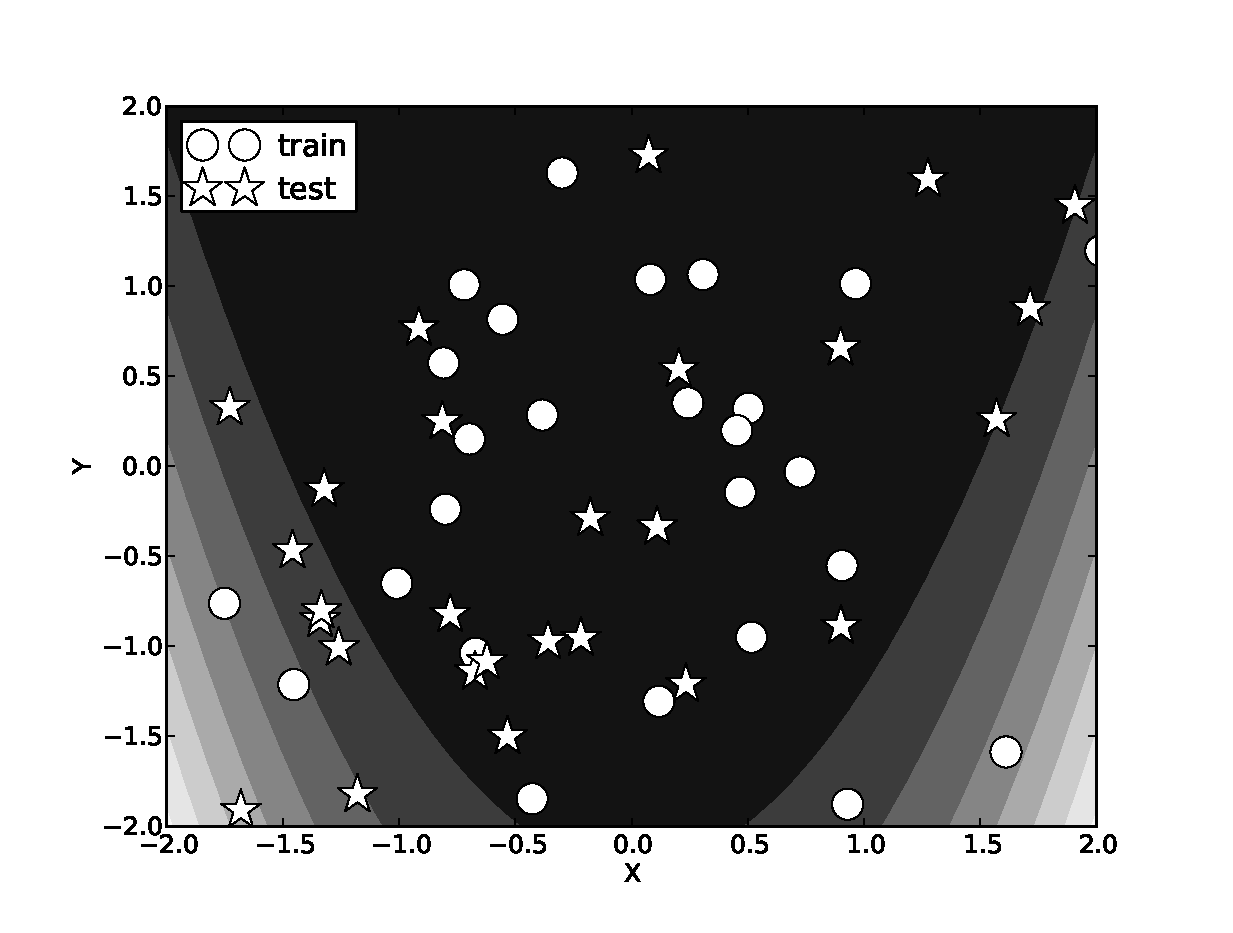
\includegraphics[width=1.0\textwidth]{SS.eps}
  \end{minipage}
  \caption[A split sampling example.]{A demonstration of split sampling using a two-dimensional Rosenbrock function.}
  \label{fig:SS} 
\end{figure}
The error estimate highly depends on the partition of available data and is thus prone to produce varied or biased estimates. Also, the testing data set does not become a part of the surrogate construction process: thus a lot of exact function evaluations are not put to good use. Split sampling  is considered belonging to methods requiring exact function evaluations to calculate the surrogate model error, since a separate set of precise observations are reserved for model validation and not used in surrogate building. 
Split sampling is the forerunner of the cross validation strategy discussed in section~\ref{sec:CV} which addresses the inefficient use of exact function evaluations,  by including all the available data for surrogate model training.






\section{Methods without Additional Exact Function Evaluations}
%A brief review of model independent error estimation is provided in Queipo~\etal~\cite{Queipo2005}.
\subsection{Bootstrapping}
Efron~\cite{BootstrapOrig} introduced bootstrapping to measure uncertainties in surrogate model predictions using three estimates: \emph{simulation, statistical, and specification errors}. 
Bootstrapping has numerous variants namely non-parametric bootstrapping, smoothed bootstrapping, and 0.632 bootstrapping~\cite{Bootstrap1,Bootstrap2}. A typical and simplest bootstrapping procedure is outlined below:
\begin{enumerate}
\item Generate a set of training data $\bm{F}(\bm{X})=\{f^{(1)},f^{(2)},\ldots,f^{(N)}\}$ from exact simulations,
\item Construct a surrogate model using the available data and evaluate the model to get the desired output $P$ (e.g. mean or variance of the exact function),
\item Generate simulated values $\widehat{f}(\x)$ from the surrogate model $\widehat{\bm{F}}(\bm{X})=\{\widehat{f}^{(1)},\widehat{f}^{(2)},\ldots,\widehat{f}^{(N)}\}$,
\item Use the simulated data as training data to construct the surrogate and re-estimate the desired output $P$.
\end{enumerate}
The above steps are repeated $m$ number of times as determined by the user and the outputs are compared to assess the model accuracy.
 
\begin{figure}[h]
\centering
\begin{minipage}[b]{0.5\linewidth}
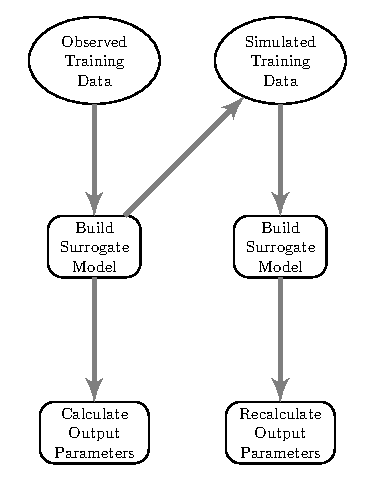
\includegraphics[width=1.0\textwidth]{BootStrapFlowchart.eps}
\end{minipage}
\caption{A sequence of steps involved in bootstrapping.}
\label{fig:GlowchartBootStrap}
\end{figure}

Bootstrapping is simple to implement and provides a measure for the stability of the results. However, the bootstrapping procedure is time-consuming and is thus not applicable for higher dimensional problems. 
For a detailed review on bootstrapping the reader is referred to works in the literature~\cite{Bootstrap1,Bootstrap2,CrossValidation2}.

%%http://www.stat.cmu.edu/~cshalizi/402/lectures/08-bootstrap/lecture-08.pdf
%he bootstrap approximates the sampling distribution, with three sources of
%approximation error. First, simulation error: using nitely many replications t%o stand for the full sampling distribution. Clever simulation design can
%shrink this, but brute force | just using enough replicates | can also make
%it arbitrarily small. Second, statistical error: the sampling distribution of
%the bootstrap re-estimates under our estimated model is not exactly the same
%as the sampling distribution of estimates under the true data-generating process% The sampling distribution changes with the parameters, and our initial
%estimate is not completely accurate. But it often turns out that distribution
%of estimates around the truth is more nearly invariant than the distribution of
%estimates themselves, so subtracting the initial estimate from the bootstrapped
%values helps reduce the statistical error; there are many subtler tricks to the
%same end. Third, specication error: the data source doesn't exactly follow
%our model at all. Simulating the model then never quite matches the actual
%sampling distribution.

\subsection{Cross Validation}\label{sec:CV}
Cross validation~\cite{CVOriginal,CrossValidation1,CrossValidation2} is a popular method to estimate a surrogate model's accuracy which does not mandate any additional function evaluations.
\subsubsection{$k$-fold Cross Validation}
In $k-$fold cross validation the data set $N$ is divided into $k$ disjoint subsets with $n$ training points in each set, and the surrogate model is constructed using the union of $k-1$ subsets of data (or equivalently $n(k-1)$ data points) and the remaining points from the left-out subset ($n$ points) are used to find the \emph{cross validation error} (CVE). The entire procedure is repeated $k$ times, each time with a different subset for validation. Thus, the whole data is used for training as well as validation, making it more attractive than split sampling.
\beq
\textrm{CVE}^{(j)}=\sqrt{\frac{1}{n}\sum_{i=1}^{n}{(f^{(i)}-\widehat{f}^{(i)})^2}}\quad\;j=1,\ldots,k,
\eeq
where $f^{(i)}$ is already available and $\widehat{f}^{(i)}$ is provided by the surrogate model.
The average error across all $k$ trials is computed as \emph{mean cross validation error},
\beq
\textrm{MCVE}=\sqrt{\frac{1}{k}\sum_{j=1}^{k}\textrm{CVE}^{(j)}}.
\eeq
A variant of this method has been proposed by Efron~\cite{CrossValidation1} to randomly divide the data into a test and training set $m$ different times and repeat the above procedure to reduce the dependency of CVE on partitioning. 


\subsubsection{Leave-one-out Cross Validation}\label{loocve}
If the number of subsets, $k$, is equal to the total number of training points, $N$, then the approach is termed \emph{leave-one-out cross validation}. In this case the surrogate model has to be reconstructed $N$ times using $N-1$ training points each time. The cross validation errors can be calculated as,
\beq
\textrm{CVE}^{(j)}={|f^{(i)}-\widehat{f}^{(i)}|}\quad\;j=1,\ldots,k,
\eeq
and
\beq
\textrm{MCVE}=\sqrt{\frac{1}{k}\sum_{j=1}^{k}\textrm{CVE}^{(j)}}=\sqrt{\frac{1}{N}\sum_{j=1}^{N}\textrm{CVE}^{(j)}}.
\eeq
%The advantage of this method is that no additional exact function evaluations are needed.
The cross-validation estimate of prediction error is nearly unbiased but can be highly variable. 
The disadvantage of this method is that the surrogate has to be constructed multiple times which can be computationally intensive as the training data size ($N$) increases.
However, having multiple approximations may improve the robustness of the whole surrogate generation and validation approach, since all available data is used for both training and testing purposes. 
For more details on cross validation the reader is referred to Efron~\etal~\cite{CrossValidation1,CrossValidation2}.

\subsection{Regional Error Estimation}
Mehmani \etal~\cite{Mehmani2012} developed a  methodology to quantify the surrogate error in different regions of the domain, which is called the regional error estimation of surrogates (REES) method. 
The REES method provides a model independent error measure that does not require any additional function evaluations. 
After segregating the domain into sub-spaces (or regions) \emph{variation of the error with sample density} (VESD) regression models are constructed to predict the accuracy of the surrogate in each subspace.
These regression models are trained by the errors (the mean and maximum error) and evaluated for the intermediate surrogates in an iterative process. 
At each iteration, the intermediate surrogate is constructed using different subsets of training points and tested over the remaining points. 
Their results indicate that the REES measure is capable of evaluating the regional performance of a surrogate with reasonable accuracy.

\subsection{Surrogate Model Inbuilt Estimates}

\subsubsection{Kriging}

The kriging prediction of a function value $\widehat{f}(\x)$ comes along with an estimate of uncertainty in prediction, \emph{the mean square error} which is shown in Figure~\ref{fig:krigingexample}. 
More details on this measure were provided in sections~\ref{MSE} and \ref{MSE2}.

\subsubsection{Gaussian Process Regression}
Gaussian process regression (GPR)~\cite{Keane2005} is similar to kriging but differs by virtue of its regression property. It also provides bounds on its prediction like kriging which is shown in Figure~\ref{fig:GPRexample}.
\begin{figure}[h]
\centering
\begin{minipage}[b]{0.48\linewidth}
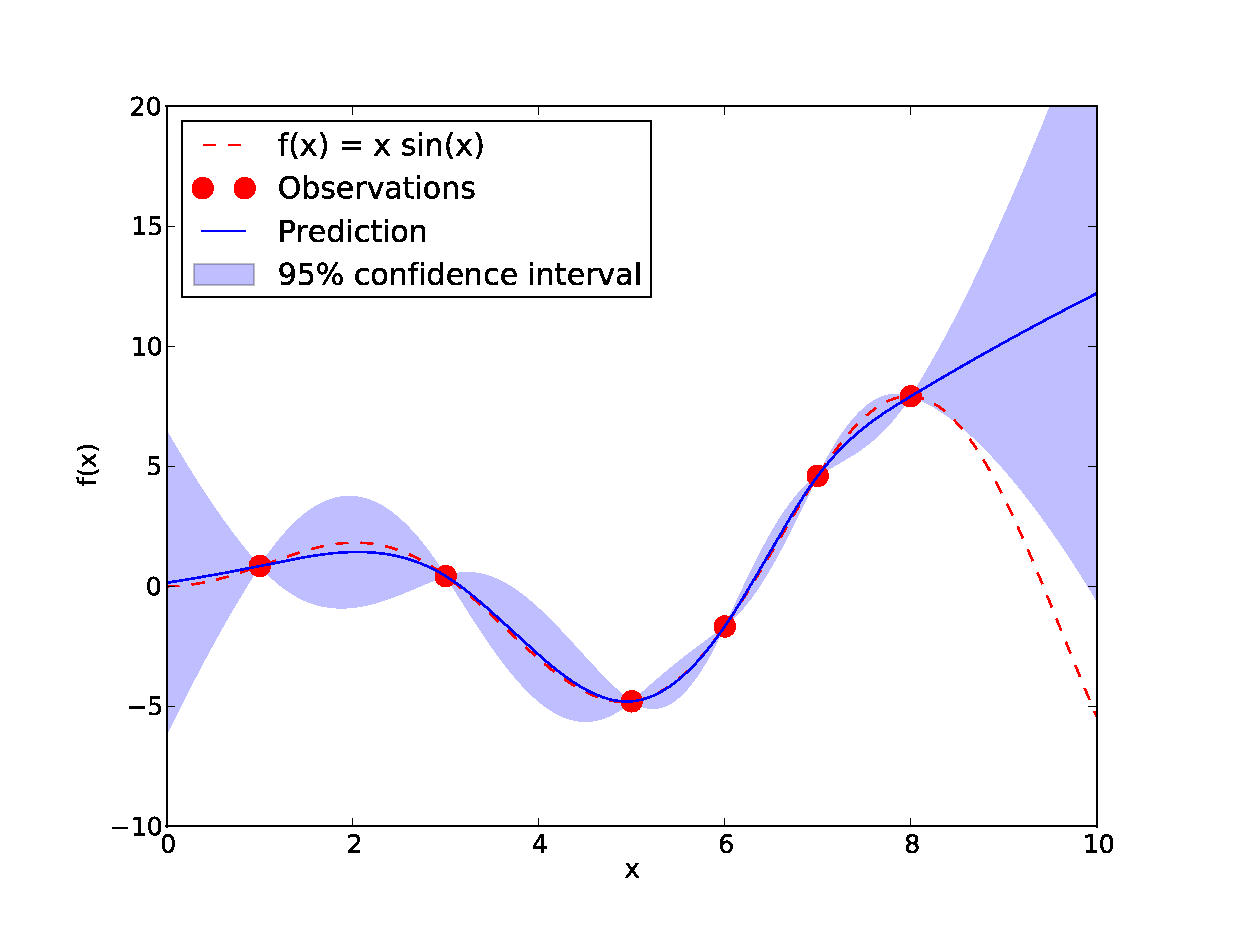
\includegraphics[width=1.0\textwidth]{figures/KrigingExample.eps} \subcaption{Kriging}
\label{fig:krigingexample}
\end{minipage}
\begin{minipage}[b]{0.48\linewidth}
   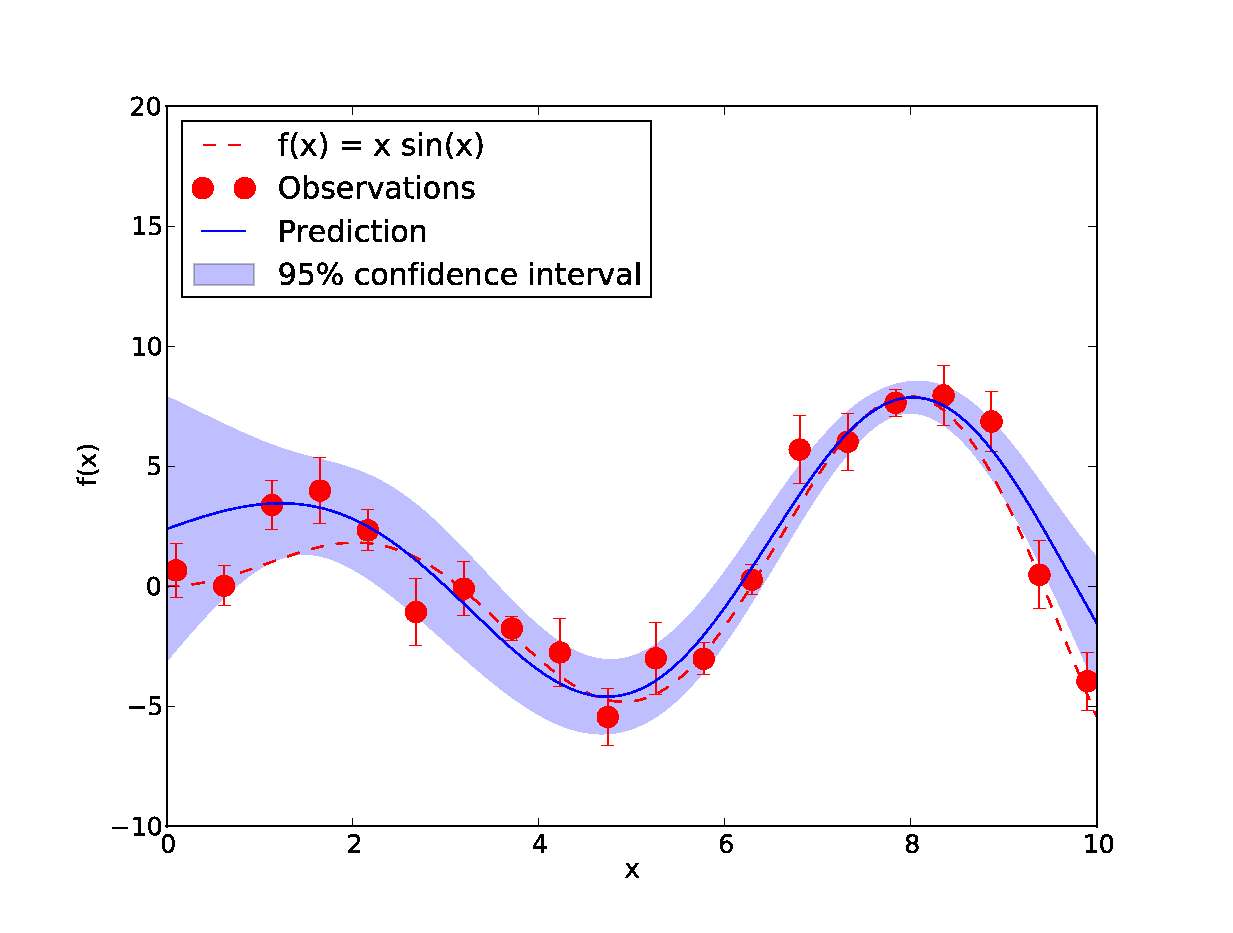
\includegraphics[width=1.0\textwidth]{figures/GPR.eps} \subcaption{Gaussian process regression}
\label{fig:GPRexample}
\end{minipage}
\caption[An illustration for confidence bounds on surrogate model predictions.]{An illustration for confidence bounds on surrogate model predictions of $f(x)=x\sin(x)$.}
\label{Boundexample}
\end{figure}
For kriging and GPR, the approximation bounds are based on statistical assumptions that errors are due to noise which follows a normal distribution with zero mean and variance $\sigma^2$.
These measures are not an approximation to the actual error but rather an uncertainty bound which is a function of distance from existing training points.


\subsubsection{Multivariate Interpolation and Regression}

Similarly, the multivariate interpolation and regression (MIR) model provides uncertainty bounds on the approximated function value as $[\widehat{f}(\x)-c\sigma(\x),\widehat{f}(\x)+c\sigma(\x)]$, where the function prediction $\widehat{f}(\x)$ and its possible deviation $\sigma(\x)$ are calculated in an equality-constrained least-squares problem~\cite{Qiqi2010a,Qiqi2010b}.



%\subsection*{Summary}
In this chapter a review of several error estimation methods, used within the surrogate modeling community to assess the accuracy of model predictions, has been provided. In spite of the presence of these methods, the main drawback among these methods are as follows:
\begin{itemize}
\item The error measurement methods discussed in section~\ref{sec:withrealevals} require additional exact function evaluations and can therefore be prohibitively expensive. 
These methods are generally only used for initial validation purposes on inexpensive analytical test functions.
\item Many parameters offer guidance on the accuracy level of the surrogate model, but mathematically they are not an actual error measure (e.g. MSE, REES). 
Moreover, many surrogate modeling approaches do not come with built-in uncertainty bounds (e.g. polynomial chaos).
\end{itemize}
The lack of a good error estimator for surrogate models in spite of their numerous practical applications has been a major motivation for this work. This has led to the development of the proposed \emph{unified training point selection and error estimation framework} requiring no additional exact function evaluations and which is applicable to any surrogate modeling approach. The details of the framework are elaborated in the following chapter.


\blfootnote{A python based data mining and data analysis tool \emph{scikit-learn}~\cite{scikit-learn} was used to produce Figures~\ref{fig:SS} and~\ref{Boundexample}.}
